\documentclass{beamer}
% \documentclass[handout]{beamer}  % removes animations
\usetheme{metropolis}
\usepackage[yyyymmdd]{datetime}
\usepackage{tikz}
\usetikzlibrary{positioning}

\renewcommand{\dateseparator}{--}

\title{VeriDash}
\subtitle{An AI-Driven, User-Centric Open Source Dashboard for Enhancing Multimedia Verification}
\date{2024--11--27}
\author{Johannes Skivdal, Laurence Dierickx, Duc-Tien Dang-Nguyen}
\institute{University of Bergen, Norway}

\renewcommand{\figurename}{Fig.}

\definecolor{nordispurple}{RGB}{26, 26, 58}
\setbeamercolor{title}{fg=nordispurple}
\setbeamercolor{title separator}{fg=nordispurple}
\setbeamercolor{frametitle}{bg=nordispurple, fg=white}

\usepackage{hyperref}
\hypersetup{
    colorlinks=true,
    linkcolor=blue,
    filecolor=magenta,
    urlcolor=cyan,
    pdftitle={presentation},
    pdfpagemode=FullScreen,
  }

% 20 minute presentation
\begin{document}
  \begin{frame}
    \maketitle

    \begin{tikzpicture}[overlay, remember picture]
      \node[above right=0.82cm and .8cm of current page.south west]{
        
\includegraphics[width=3cm]{figures/UiB_Positiv2linjer.png}
      };

      \node[above =1cm of current page.south]{
        
\includegraphics[width=3cm]{figures/nordis-logo.png}
      };
    \end{tikzpicture}
  \end{frame}

  \begin{frame}{What}
    Verification $\neq$ Fact Checking!
    \begin{itemize}
      \item Fact Checking: long invesigative work, "surgeon"  % journalistic skill required
      \item Verification: sanity check of breaking news, "first aid"
    \end{itemize}

    VeriDash is:
    \begin{itemize}
      \item Creating a single User Interface for Video Verification
      \item Combining off-the-shelf tools
      \item Facilitating faster human work
    \end{itemize}
  \end{frame}

  \begin{frame}{Why}
    Twain: \textit{"A lie can travel halfway around the world while the truth is still putting on its shoes."}

    Journalism needs AI to handle an overwhelming amount of information

    The virality of news require ever faster verification
  \end{frame}

  \begin{frame}{VeriDash tools}
    Some essential video tools in one place:
    \begin{itemize}
      \item Audio Transcription and Translation
      \item Metadata Extraction
      \item Geolocation
      \item Frame Extraction
      \item Object Detection
      \item Frame Stitching (Overview)
    \end{itemize}

    VeriDash \textbf{does not} do:
    \begin{itemize}
      \item Automated Verification  % human-in-the-loop is important
    \end{itemize}
  \end{frame}

  \begin{frame}
    \centering
    \textbf{Demo}
  \end{frame}

  \begin{frame}{How does it work?}
    Built for modularity and scale:
    \begin{itemize}
      \item {
        Parallel \textit{job} processing: Python \& Celery  % notion of a "job"
        \begin{itemize}
          \item Job dependency modeling
        \end{itemize}
      }
      \item Live updates between server and client: WebSockets
      \item Heavy usage of caching: job results, video uploads
      \item File storage with MinIO (S3 API)
      \item Frontend: modular and interactive, React
    \end{itemize}
  \end{frame}

  \begin{frame}
    \begin{figure}
      \centering
      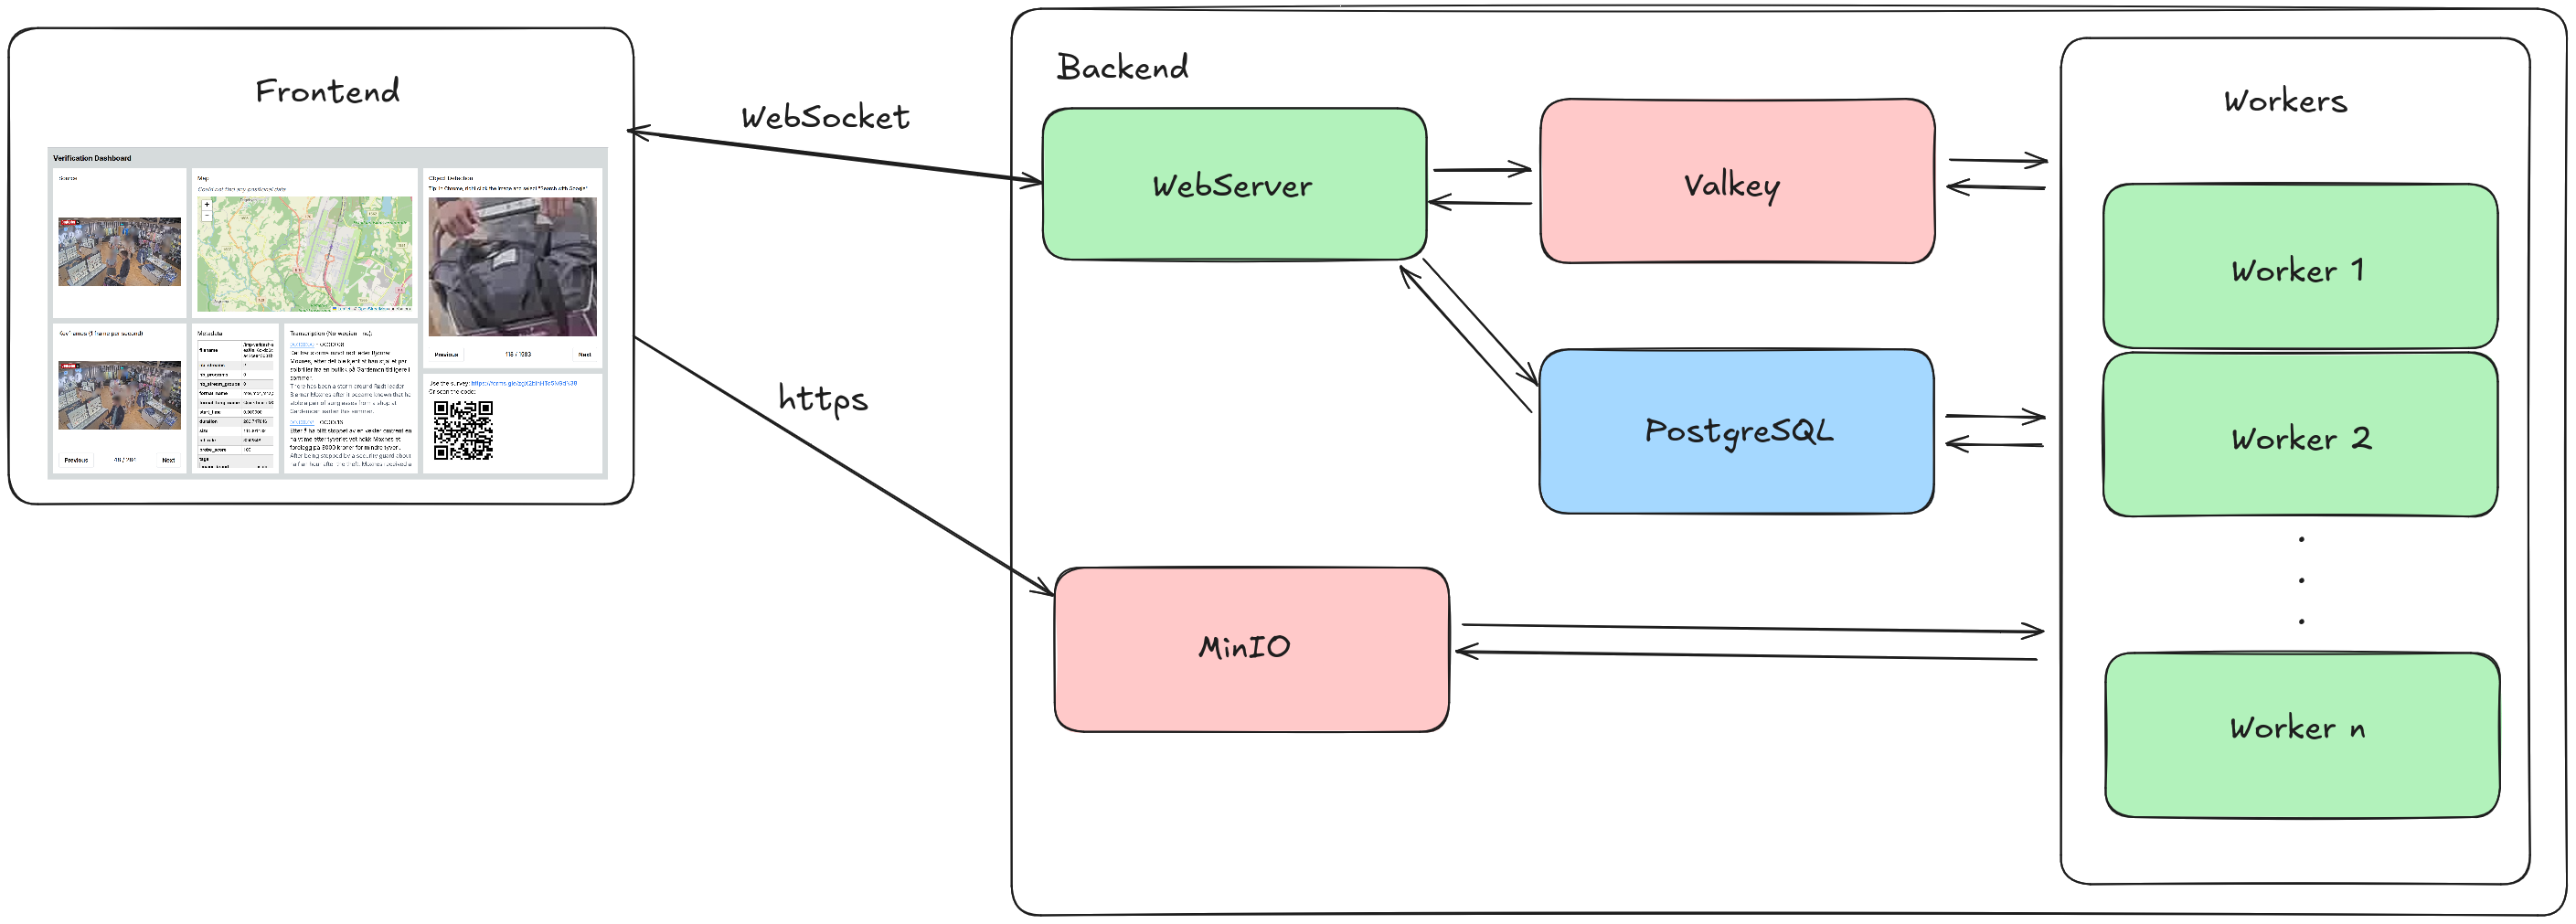
\includegraphics[width=\textwidth]{figures/veridash-system-architecture.png}
      \caption{VeriDash System Architecture Overview}
    \end{figure}
  \end{frame}

  \begin{frame}{The future}
    \begin{itemize}
      \item Nothing is set in stone, we can still replace parts etc.
      \item {
        Open-Source and designed to be extensible
        \begin{itemize}
          \item Built using industry-standard tools
          \item Just add a new job type, handlers, and UI
        \end{itemize}
      }
    \end{itemize}

    Features we want to add:
    \begin{itemize}
      \item Google Maps Street View
      \item Searchable Object Detection
      \item {
        OpenStreetMap tags-based Geolocation
        \begin{itemize}
          \item \href{https://github.com/bellingcat/osm-search}{github.com/bellingcat/osm-search}
        \end{itemize}
      }
      \item and more...
    \end{itemize}
  \end{frame}

  \begin{frame}
    \centering
    \textbf{Thank you!}

    Ideas or contributions are welcome: \href{https://github.com/skivdal/veridash}{github.com/skivdal/veridash} \\
    or: \href{mailto:johannes.skivdal@student.uib.no}{johannes.skivdal@student.uib.no}
  \end{frame}
\end{document}

